
\chapter{System Architecture}  

\section{System Overview}

\section{Fine-tuning}

The Large Language Models (LLM) used for this paper are pre-trained, meaning that the model learned how words relate to each other, the model is trained to understand a language. This process is computationally expensive and requires a large amount of data. Instead of creating a model from scratch, we can teach an existing model to learn a new task such as text classification, translation, generation, or other. This is called fine-tuning, and in this case, it was used to teach the model to classify two types of texts: health-related and misinformation-related. 
\newline
\newline
The health-related dataset comprises over 12,441 tweets extracted from the previous THS project. Said dataset was classified into three categories: related, unrelated, and ambiguous tweets. A second dataset, with 8,762 texts, was created with data from different sources such as news, social media, and blogs classified as misinformation and non-misinformation \textbf{\textit{[Insert References]}}. 

The models used for the classification process were Bert, T5, and LLaMa-2. 

\subsection{Health-Related Classification}


\subsection{Misinformation Classification}


2. Misinformation classification

LR, Batch size, seed, and epochs are static.

- Each model was fine-tune twice.

    1. Sequence classification: 1, 2, or 3; 1 or 2.

    2. Classification with text generation: Related, Unrelated, or Ambiguous; Misinformation or Not Misinformation.

- Weighted average added for the sequence classification.


\section{Paper ETL Pipeline}

Our model must use credible sources of information to rebut misinformation. We identified PubMed \textbf{[REFERENCES]}, an online library that contains peer-reviewed medical literature. We want to extract the papers and store them in a vector database. To extract these papers, we used the BioC API \cite{bioinformatics}, which has access to the PubMed library. However, the API needs the research paper's identifier, known as PubMed Central (PMC) ID. We design a scraper to extract these identifiers from the official PubMed site. The pipeline in Figure \ref{fig:etl} shows the processes of data extraction. 

\begin{figure}[!ht]
	\begin{center}
		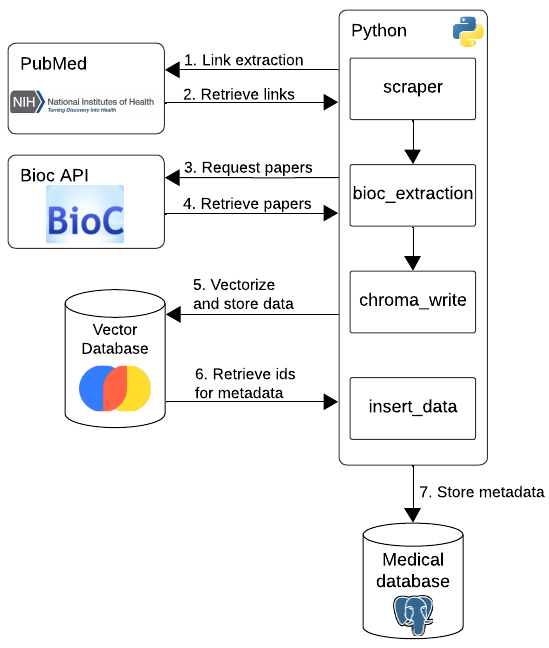
\includegraphics[width=0.75\textwidth]{images/ETL_Pipeline.png} %specify width
	\end{center}
	\caption{Medical Data Extraction Pipeline} %specify caption
	\label{fig:etl}
\end{figure}

\subsection{Scraper}
The first step of the pipeline was identifying what papers we needed to extract. We selected 17 topics for the data extraction process. These topics are:
\begin{multicols}{2}
\begin{itemize}
	\item{allergy}
	\item{bird flu}
	\item{cancer}
	\item{chickenpox}
	\item{common cold}
	\item{conjunctivitis}
	\item{covid sickness}
	\item{covid symptoms}
	\item{covid treatment}
	\item{covid vaccine}
	\item{flu vaccine}
	\item{headache}
	\item{influenza}
	\item{monkeypox}
	\item{stomach aches}
	\item{swine flu}
	\item{zika}

\end{itemize}

\end{multicols}

To extract them, we built a scraper in Python using Selenium and BeautifulSoup libraries. We used Selenium to retrieve the web source from PubMed's website, and BeautifulSoup was used to get the links to each paper. These links contained the PMC identifier. For each topic, we selected 5,000 PMC identifiers. These identifiers were grouped by topic and stored locally in Comma Separated Value (CSV) files.

\subsection{BioC API}
After retrieving those identifiers, we need to extract the research papers. Using the PubMed API, BioC, we made requests that returned the documents as JSON. These JSONs were processed to contain texts, and we removed tables and figures. Later, the paper's sections -introduction, methodology, results, and others- were combined as one attribute, excluding references. We removed tables, figures, and references from the context to ensure the chunking process worked appropriately. If the data is not processed, when performing RAG, we can retrieve data that is not useful. After that, we turned the result into a new JSON that contained the research metadata and its context. 

\subsection{Vectorizing data}
Later, each research paper’s context was split into chunks using LangChain. Then, we used an LLM, BAAI \cite{bge_embedding}, to embed these chunks. A universal unique identifier (UUID) was combined with each chunk and stored in a Chroma \cite{chroma} database. After uploading the data to Chroma, we added these UUIDs to their JSON. 


\subsection{Store metadata}
Now, with all papers vectorized, we upload the metadata into a Postgres database. First, we validate that there are no duplicate records in the system. To prevent duplicates, we search for the paper's reference. If any is found, we delete the chunks from the vector database. Additionally, any research that did not contain at least an abstract was removed. That ensures that there is no repetition or inconsistency when doing the rebuttal. Later, we upload this data into the system following the schema found in Figure \ref{fig:table}. The tables in this schema are as follow:

\begin{description}
	\item{\textbf{Research:}}  The table contains the research paper data. Its attributes are title, which is the research paper title; context, the paper’s text; paper\_ref, the complete reference of the paper, used to prevent duplicates; and fullpaper, which is a boolean that is true if the paper contains an abstract, introduction, methodology, discussion, conclusion, and references.
	\item{\textbf{Chunks:}} This table pairs the UUIDs from the paper's chunks and their respective research record.  
	\item{\textbf{Keyword:}} Some research papers contain keywords that allow the reader to know the subjects mentioned in the paper. 
	\item{\textbf{Author:}} Stores the first and last names of all authors identified in the research paper. 
	\item{\textbf{Reference:}} All references that are present in the research paper.
	\item{\textbf{Topic:}} This contains the different topics used to search the papers.

\end{description}

\begin{figure}[H]
	\begin{center}
		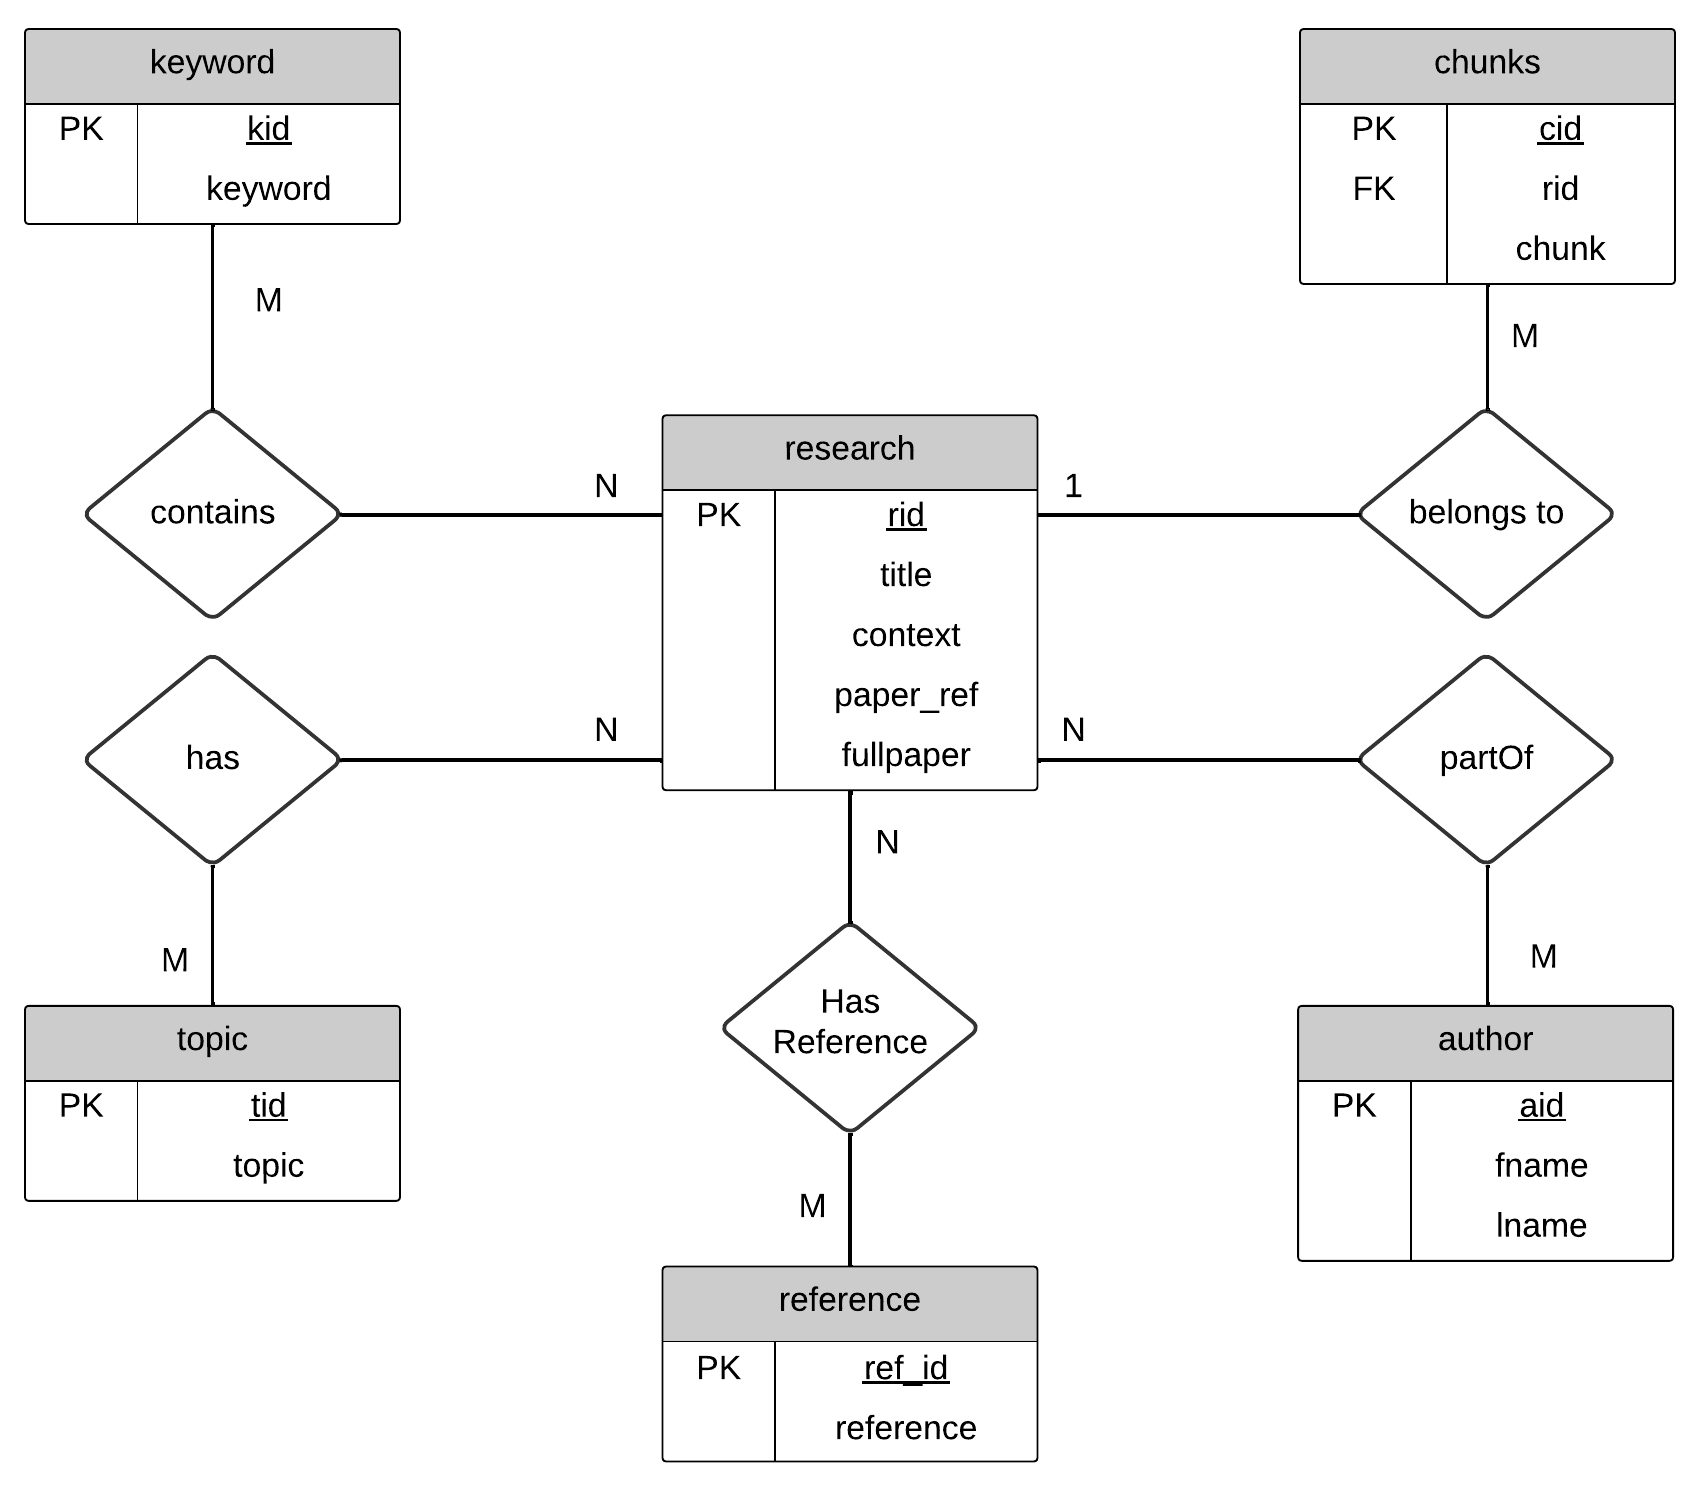
\includegraphics[width=0.9\textwidth]{images/Table_diagram.png} %specify width
	\end{center}
	\caption{Research Papers Schema Diagram} %specify caption
	\label{fig:table}
\end{figure}


We started the search with 85,000 peer-reviewed papers. After finishing the filtering and data cleaning, we ended with 56,365 different research papers. 

%- Save links in temporary file and upload to a consumer to 
%process link information.

%- Data is divided into different tables

%- Papers context is broken into chunks and uploaded into a vectored database.

%- Chunks are mapped to relational database metadata.
   % + Add ERD Schema
    
%- LLM sends query into vector database.

%- Id and context is retrieved and process. Id is sent to relational database to retrieve source.

%- Model respond with full rebuttal and official link.
   % + Add pipeline image

\section{Misinformation Rebuttal Pipeline}

The pipeline shown in Figure \ref{fig:llm} goes as follows:

\begin{enumerate}
	\item Health-related classification: Verifies if the inputted text is health-related. The possible options are related, unrelated, or ambiguous.
	\item Misinformation classification: If the text was classified as health-related, we then checks if the text contains misinformation. If any misinformation is detected, we need to find official health data to rebut said misinformation.
	\item	Context finder: A query is created for a vector database based on the original text. This query is sent to a vectorized database, Chroma, and will return chunks that are related to the query.
	\item	Medical information database:  This is a database that contains medical metadata from official sources. Using the chunk IDs we will retrieve the original papers' references.
	\item	Organize and rebut: The result from the medical database is now processed and used to make a rebuttal for the misinformation in the text. Then, we query the relational database to extract the references of the papers used for the previous part.
	The output includes the original text, the health and misinformation classifications, the correction of the misinformation, and the citation of the sources used. 
\end{enumerate}

\begin{figure}[H]
	\begin{center}
		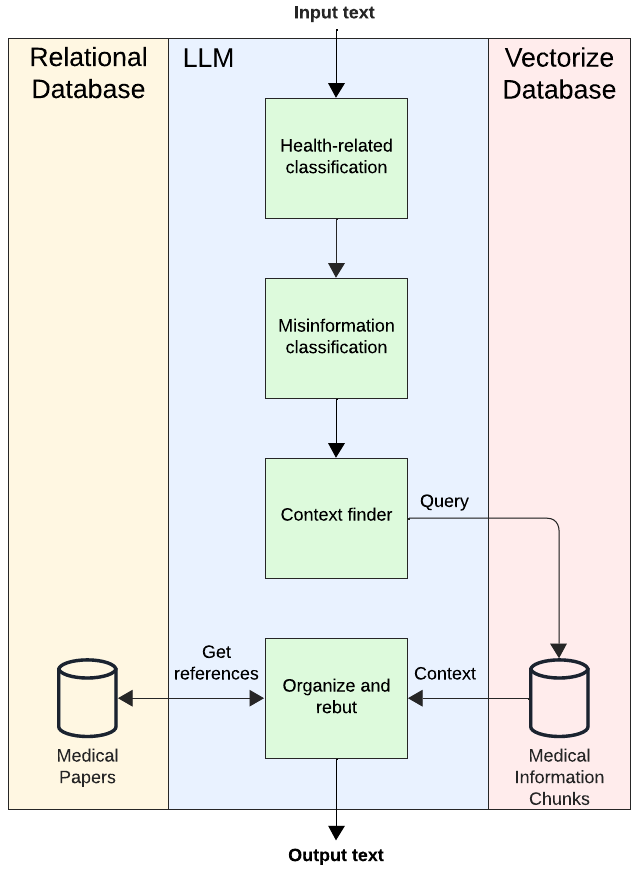
\includegraphics[width=0.75\textwidth]{images/LLM_Pipeline} %specify width
	\end{center}
	\caption{Misinformation Rebuttal LLM System Architecture} %specify caption
	\label{fig:llm}
\end{figure}

\section{Hardware and Software}
\list{-}
    \item V100 machines: 32Gb VRAM, and 80-ish RAM
    \item Cuda 11.7
    \item Python 3.9.19
    \item Pytorch 2.0.1
    \item Transformers 4.34.0

